\section{Process Background}
  The term \textit{tomography} is derived from the Greek word \textit{tomos}, which translates to \textit{slice} or \textit{section}. In the medical field, CT scans (computed tomography) combine many 2-D images from X-ray scans to generate a three-dimensional reconstruction of bodily organs. Building on this, proton tomography harnesses many nuclear reactions to reconstruct multi-dimensional mappings of partons' spatial and momentum distributions inside nucleons. 


    \subsection{Wigner Functions, Generalized Parton Distributions}

        In classical mechanics, a particle can be completely described by its position in its six-dimensional phase space (three spatial and three momentum coordinates). An ensemble of such particles can be most completely understood through its phase space distribution function, which contains the probability of finding a particle in a particular region in phase space. In quantum systems, a pure phase space distribution is not well defined because of Heisenberg's uncertainty principle. However, in 1932 Eugene Wigner introduced a formalism that addressed this \parencite{Wigner1932OnEquilibrium}, yielding functions that provide the most comprehensive representation achievable for quantum systems.
        
        
        \subsubsection*{Wigner Quasi-probability Distributions}
             Wigner Quasi-probability Distributions, commonly referred to as simply Wigner functions or Wigner distributions, are defined as in \eqref{eq:wigner_dist}. This can be integrated over \textit{x}(\textit{p}) to yield momentum (space) density, but for arbitrary (\textit{x},\textit{p}) the distribution can take negative values, and so violates probability axioms and thus is a quasi-probability distribution rather than a full probability distribution. Wigner distributions are useful outside of particle physics, notably in signal processing, with more details available in \parencite{Hillery1984DistributionFundamentals}.

             \begin{equation}\label{eq:wigner_dist}
                W(x,p) = \frac{1}{\pi\hbar} \int_{-\infty}^{\infty} \psi^\times (x+\eta) \psi(x-\eta) e^{2ip \eta/\hbar} d\eta.
            \end{equation}\myequations{Wigner Quasi-probability Distributions}

        
             %In simple systems Wigner distributions can be and have been directly measured,  

            The corresponding generalization to relativistic quark and gluon phase space distributions is covered in \parencite{Ji2004GENERALIZEDDISTRIBUTIONS} to yield a Wigner Operator \eqref{eq:wigner_operator} which can be used to obtain the reduced quantum phase-space quark distributions in the nucleon \eqref{eq:wigner_reduced}. 

            \begin{equation}\label{eq:wigner_operator}
                \hat{W}_{\Gamma}(\Vec{r},k) = \int_{-\infty}^{\infty} e^{ik\cdot\eta} \Bar{\Psi}(\Vec{r}-\eta/2) \Gamma \Psi(\Vec{r}-\eta/2)  d^4\eta
            \end{equation}\myequations{Wigner Operator}

            \begin{equation}\label{eq:wigner_reduced}
                     W_{\Gamma}(\Vec{r},\Vec{k}) = \int \frac{dk^-}{4\pi^2} \frac{1}{2}   \int \frac{d^3\Vec{q}}{8\pi^3}  e^{-i\Vec{q}\cdot\Vec{r}} \bra{\Vec{q}/2} \hat{W}_{\Gamma}(\Vec{r},k)\ket{-\Vec{q}/2}.
            \end{equation}\myequations{Reduced Wigner Distribution}

            Here we have integrated over $k^- = (k^0-k^z)/\sqrt{2}$, the light-cone energy, since it is difficult to measure in high-energy processes. 
    
    
        \subsubsection*{Generalized Parton Distributions}\label{sec:ch1sec2GPDs}

            \todo{possibly work in TPEX by discussion of OPE formalism}
            \todo{if possible work in Operator Product and Twist expansion}
            
            No known experiments currently exist that are able to directly measure this distribution (nor is it known if it is possible). Fortunately, in recent decades theorists have been able to link experimental observables to further reduced forms of \eqref{eq:wigner_reduced}. Specifically, integration can be performed over spatial coordinates to yield Transverse Momentum Distributions (TMDs) which are outside the scope of this work. Alternatively, integration can be performed over momentum coordinates to yield Generalized Parton Distributions (GPDs), which encode transverse spatial as well as longitudinal momentum distributions of partons inside the nucleon. As shown in \parencite{Ji2004GENERALIZEDDISTRIBUTIONS}, at leading-twist (twist-2), iterating through all choices of the Dirac matrix for quark distributions $\Gamma$ yields eight distinct GPDs for every quark flavor. They are generally expressed in terms of parton momentum fraction \textit{x}, skewness $\xi = \frac{-q^2}{q \cdot P} \sim \frac{x_B}{2-x_B}$, and momentum transfer \textit{t}.
            
            Four GPDs correspond to helicity conserving (chiral even) processes and four correspond to helicity flipping (chiral odd) processes: \GPDH,  \GPDE,  \GPDHtilde,  and \GPDEtilde  \quad for chiral even, and \GPDHT,  \GPDET,  \GPDHTtilde, and \GPDETtilde \quad (\GPDETbar = 2*\GPDHTtilde+\GPDET is commonly used). Table \ref{table:GPDsPolarization} summarizes the GPDs with respect to polarization states. 
        
            %\textcolor{red}{    Why do the scrtucture combine in the way they do with the coefficents of cos phi terms and epsilons? - insert old links from papers from 1980s}
            
            \begin{table}[H]
                
                \centering
                \begin{tabular}{@{} *{4}{c} @{}}
                        \headercell{Nucleon \\ Polarization} & \multicolumn{3}{c@{}}{Quark Polarization}\\
                        \cmidrule(l){2-4}
                        & U & \textcolor{white}{lllll}L & T    \\ 
                        \midrule
                          U  & \GPDH &               *                    &  \GPDETbar = 2\times \GPDHTtilde+\GPDET  \\
                          L  &    *                &  \textcolor{white}{llll}\GPDHtilde &     \GPDETtilde                           \\
                          T  & \GPDE &               \GPDEtilde                   &  \GPDHT,\GPDHTtilde \\
                    \end{tabular}\\
        
                    
                    \caption[GPDs Across Nucleon and Quark Polarizations]{GPDs Across Nucleon and Quark Polarizations.  * forbidden by parity.}
                    \label{table:GPDsPolarization}
            \end{table}

            GPDs can be understood by considering further integrations and forward limits. In the same way that the nucleon charge must be recovered when integrating over PDFs or Form Factors, these functions themselves are recovered when appropriately integrating over GPDs, as in \figref{fig:gmtd_cube}. Specifically, first moments of the GPDs $H$ and $E$ are related to the Dirac and Pauli form factors $F_1$ and $F_2$ respectively:
        
            \begin{figure}[H]
                \centering
                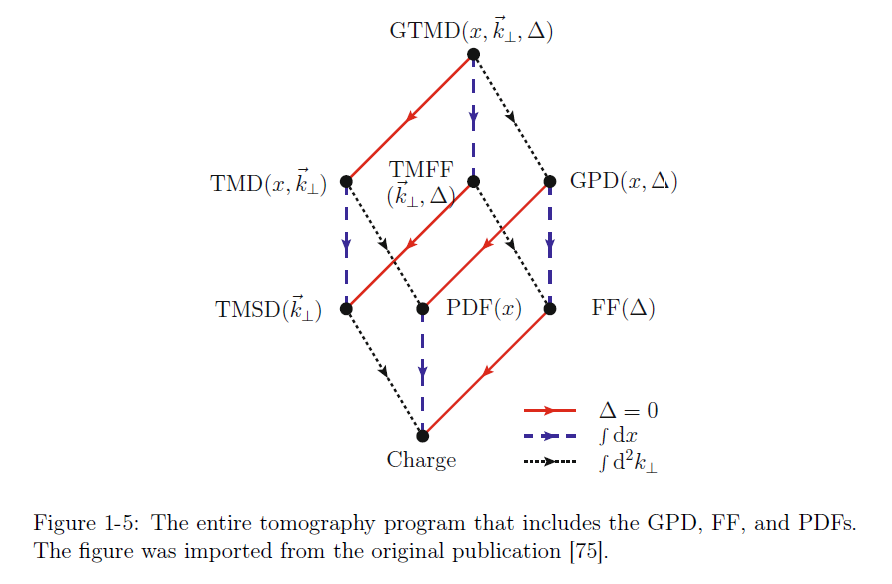
\includegraphics[width=0.55\textwidth,trim={3cm 1.5cm 3cm 0},clip]{Chapters/Ch1-Intro/Ch1-Sec2-GPDs-DVMP/pics/gtmd-cube-sangbaek.png}
                \caption[Distribution Relationship Cube]{Relation cube, from \parencite{Burkardt2016ModellingStructure}. }
                \label{fig:gmtd_cube}
            \end{figure}
        
        \begin{equation}\label{gpd_f1}
        \int dx \, H(x, \xi, t) = F_1(t)
        \end{equation}
        
        \begin{equation}\label{gpd_f2}
        \int dx \, E(x, \xi, t) = F_2(t). 
        \end{equation}


        GPDs have been shown \parencite{Ji1997Gauge-InvariantSpin} to encode spin distributions and also can be interpreted as describing the transverse spatial distribution of quarks \parencite{Burkardt2007GPDs0}. Further, GPDs' relation to energy-momentum tensor form factors (EMTs) allows access to EMT densities, which describe the distribution of energy, momentum, and pressure inside the nucleon. It was originally not known how to measure GPDs, but later were found to be experimentally accessible through deeply virtual exclusive processes (DVEP) relying on factorization theorems \parencite{Collins1999ProofQCD}, \parencite{Bauer2002HardTheory}. 
           
    
    
    \subsection{Deeply Virtual Exclusive Processes}

        Deeply virtual exclusive processes are interactions occurring with high photon virtuality $(Q^2  \gg  m_p^2$) in the DIS regime ($W^2 \gg m_p^2$), with thresholds normally set to require  $Q^2 > 1$ GeV$^2$ and $W>2$ $GeV$. The processes involve the scattering of a virtual photon off a nucleon target, yielding either a real photon or mesons, along with an intact final state nucleon and incident particle (e.g. from an electron or muon beam). These processes are in stark contrast to DIS, where the nucleon target is shattered into many pieces, and can instead be thought of as a hard yet precise non-invasive process. Different reactions have been shown to have different GPD dependencies, and thus provide different windows into sub-nucleon mechanics. 

        \subsubsection*{Deeply Virtual Compton Scattering and Meson Production}
        \figref{fig:dvep_diagram} illustrates diagrams for Deeply Virtual Compton Scattering (DVCS) and Deeply Virtual Meson Production (DVMP). 
    
        \begin{figure}[H]
            \centering
            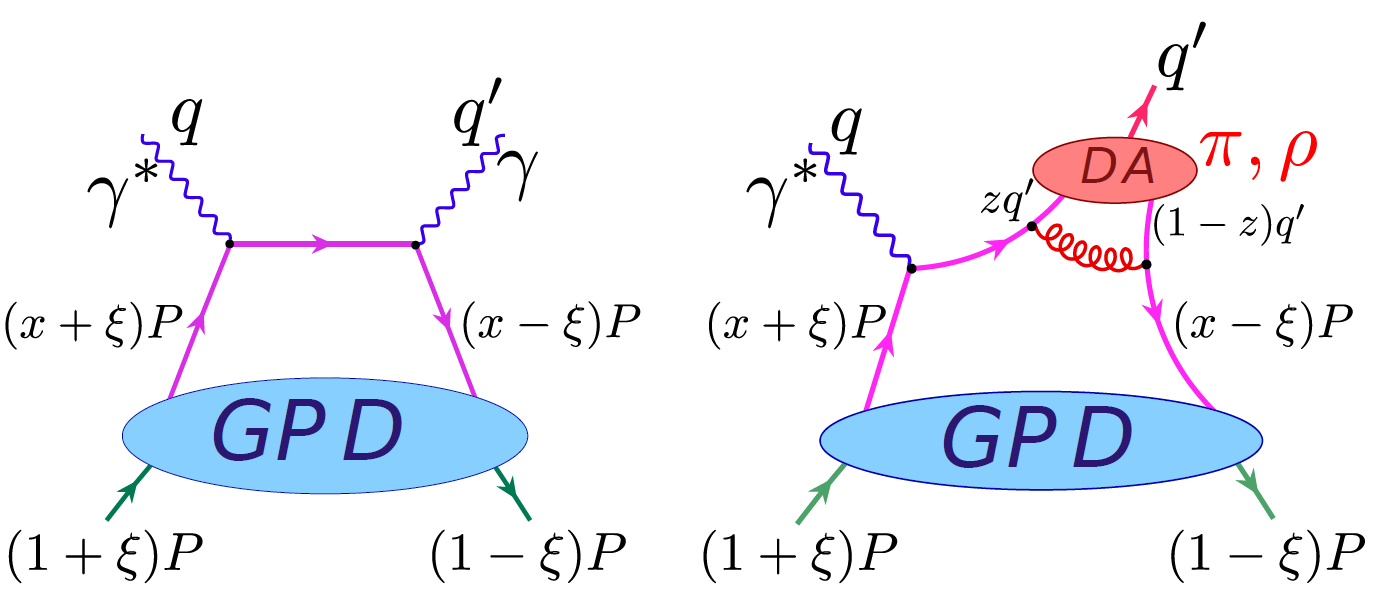
\includegraphics[width=0.8\textwidth]{Chapters/Ch1-Intro/Ch1-Sec2-GPDs-DVMP/pics/valery_dvep.png}
            \caption[DVCS and DVMP Feynman Diagrams]{Feynman diagrams for DVCS (left) and DVMP (right), from  \parencite{Kubarovsky2011DeeplyCLAS}. DA refers to the appropriate meson distribution amplitude.}
            \label{fig:dvep_diagram}
        \end{figure}

        DVCS is widely regarded as the ``cleanest '' channel and has already been leveraged to provide great insights into the structure of the nucleon. For example, \figref{fig:proton_pressure_exp} shows the pressure distribution inside a proton from DVCS data \parencite{Burkert2018TheProton}, which has since been further investigated by theorists to generate similar mappings through LQCD as in \figref{fig:proton_pressure_theory}

        \begin{figure}[H]
        \centering
        \begin{minipage}{0.48\textwidth}
            \centering
            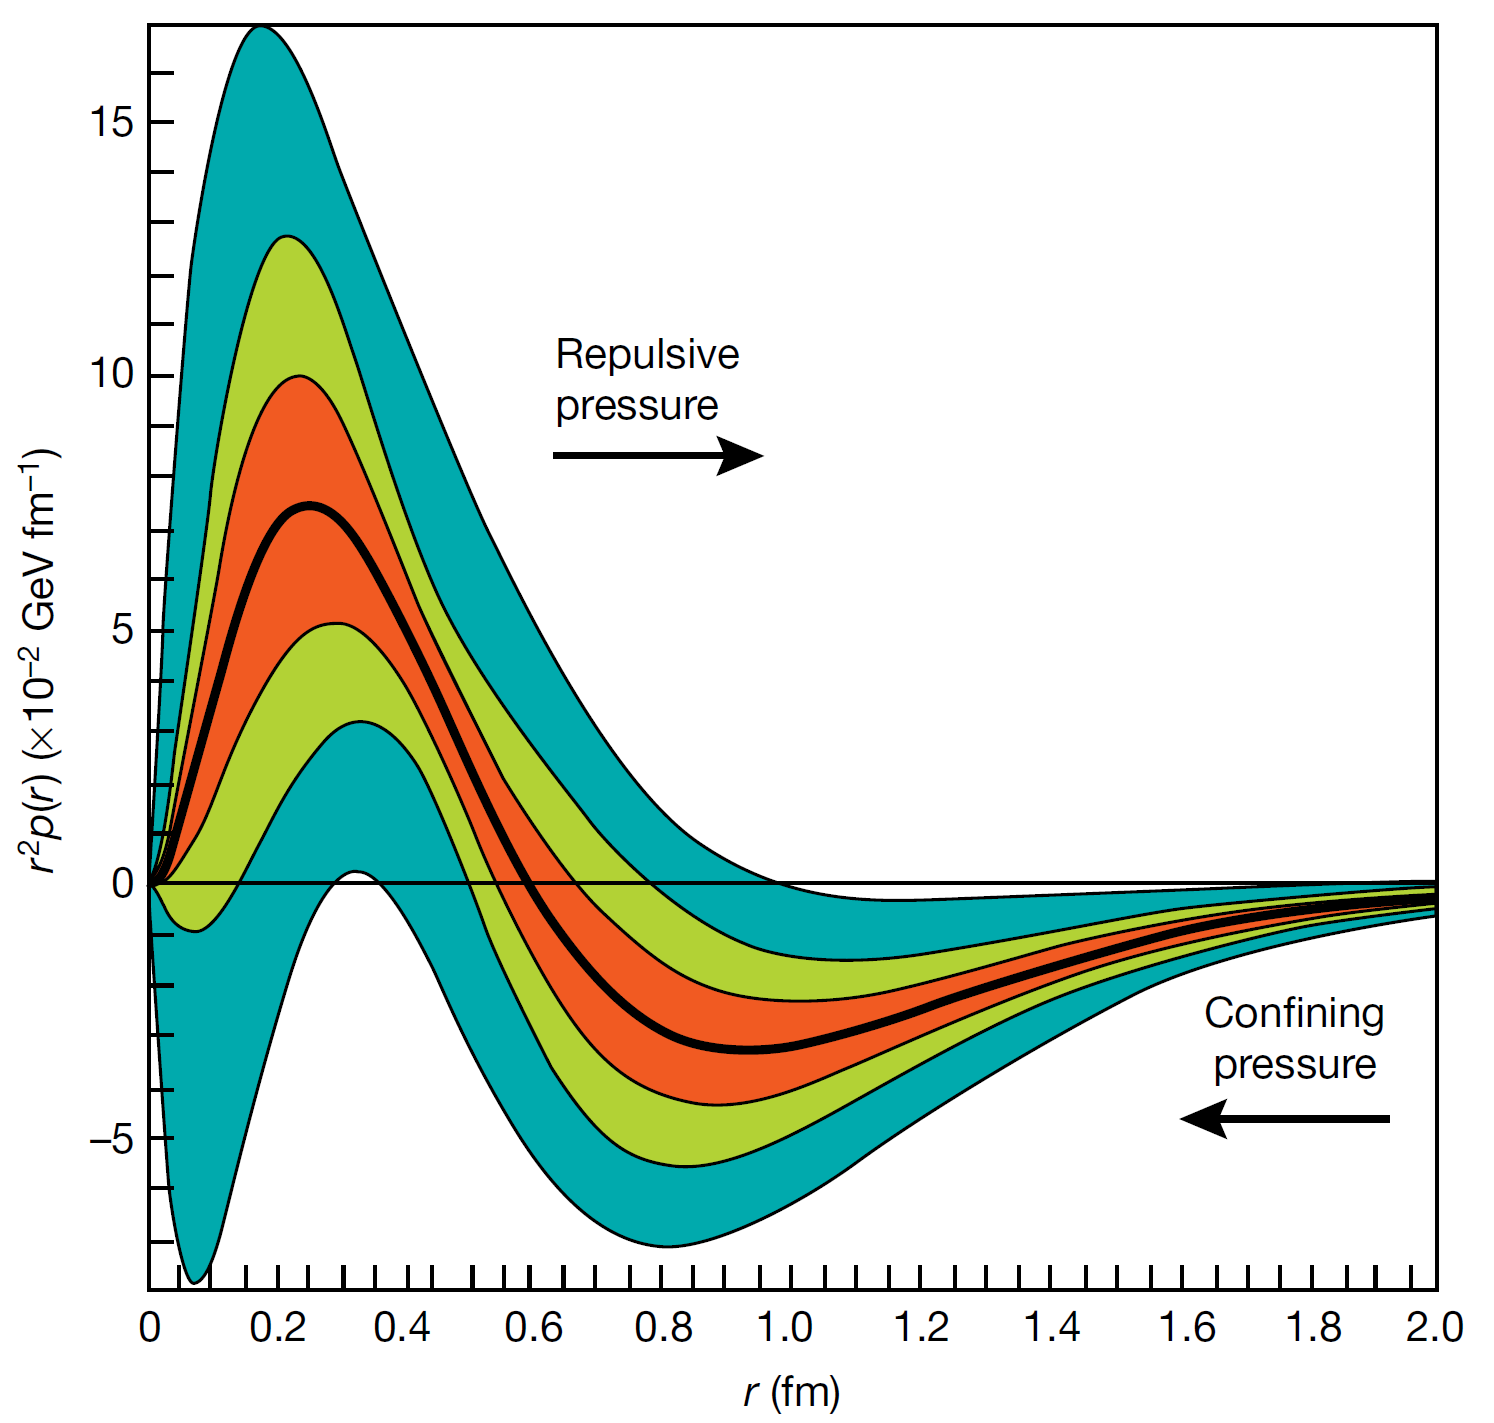
\includegraphics[width=0.65\textwidth]{Chapters/Ch1-Intro/Ch1-Sec2-GPDs-DVMP/pics/proton_pressure_dist.png}
            \caption[Proton Pressure Distribution, Experiment]{Proton Pressure Distribution from DVCS data, from \parencite{Burkert2018TheProton}.}
            \label{fig:proton_pressure_exp}
        \end{minipage}\hfill
        \begin{minipage}{0.48\textwidth}
            \centering
            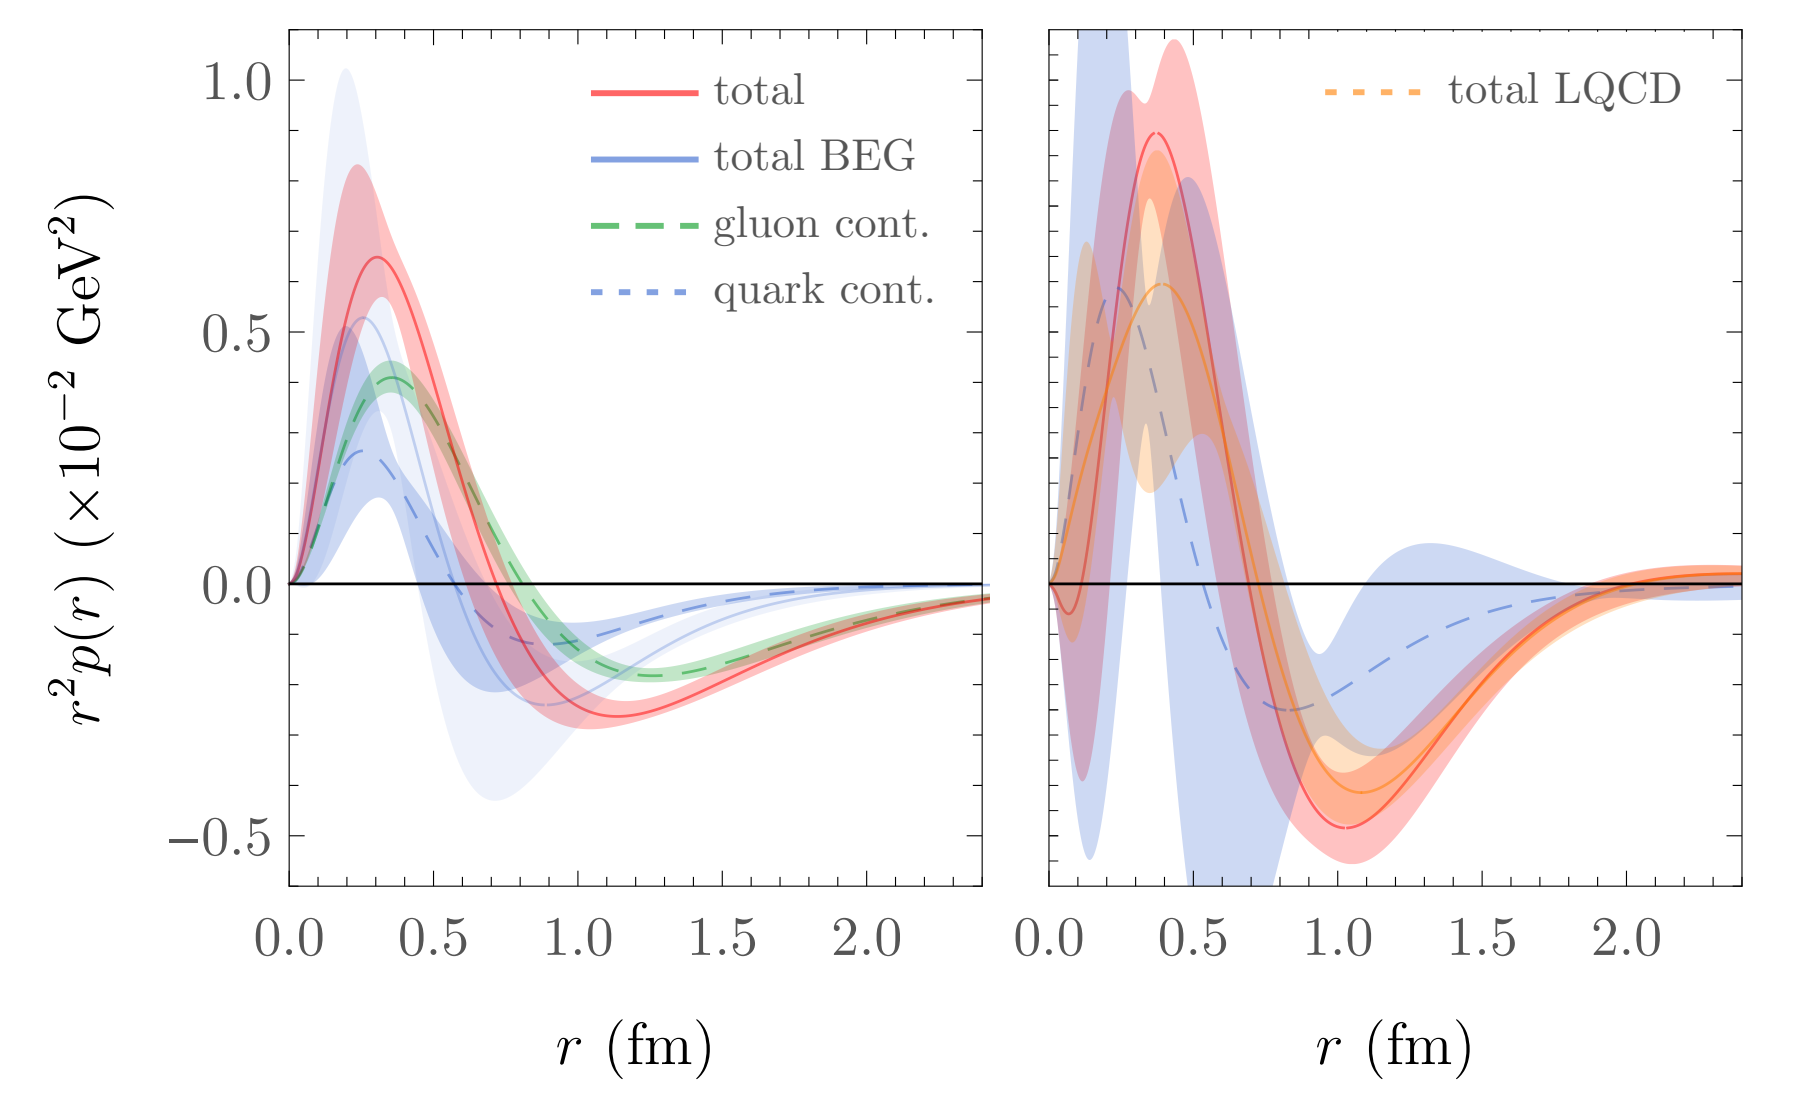
\includegraphics[width=0.99\textwidth]{Chapters/Ch1-Intro/Ch1-Sec2-GPDs-DVMP/pics/proton_pressure_theory.png}
            \caption[Proton Pressure Distribution, Theory]{Proton Pressure Distribution from Lattice QCD, from \parencite{Shanahan2019PressureProton}.}
            \label{fig:proton_pressure_theory}
        \end{minipage}
    \end{figure}

        DVCS is primarily sensitive to non-quark spin flip GPDs (e.g. \GPDH, \GPDE), as are DVMP for vector mesons, such as the $\rho$. On the other hand, pseudoscalar meson production, such as pions, are sensitive to the transversity, or chiral-odd, GPDs. Additionally, some meson processes, such as $\phi$ due to its strange quark content, are particularly sensitive to gluon GPDs. This work focuses on DVMP with the production of a neutral pion, $\pi^0$, which in addition to accessing chiral-odd GPDs, is an important background for other processes such as DVCS due to sample contamination from $\pi^0$ decay \parencite{Lee2022MeasurementDetector}.
        
        \subsubsection*{Deeply Virtual Neutral Pion Production}
            The Feynman diagram for Deeply Virtual Neutral Pion Production (DV$\pi^0$P or DVPiP) is shown in \figref{fig:DVPiP_diagram}. 

            \begin{figure}[H]
                \centering
                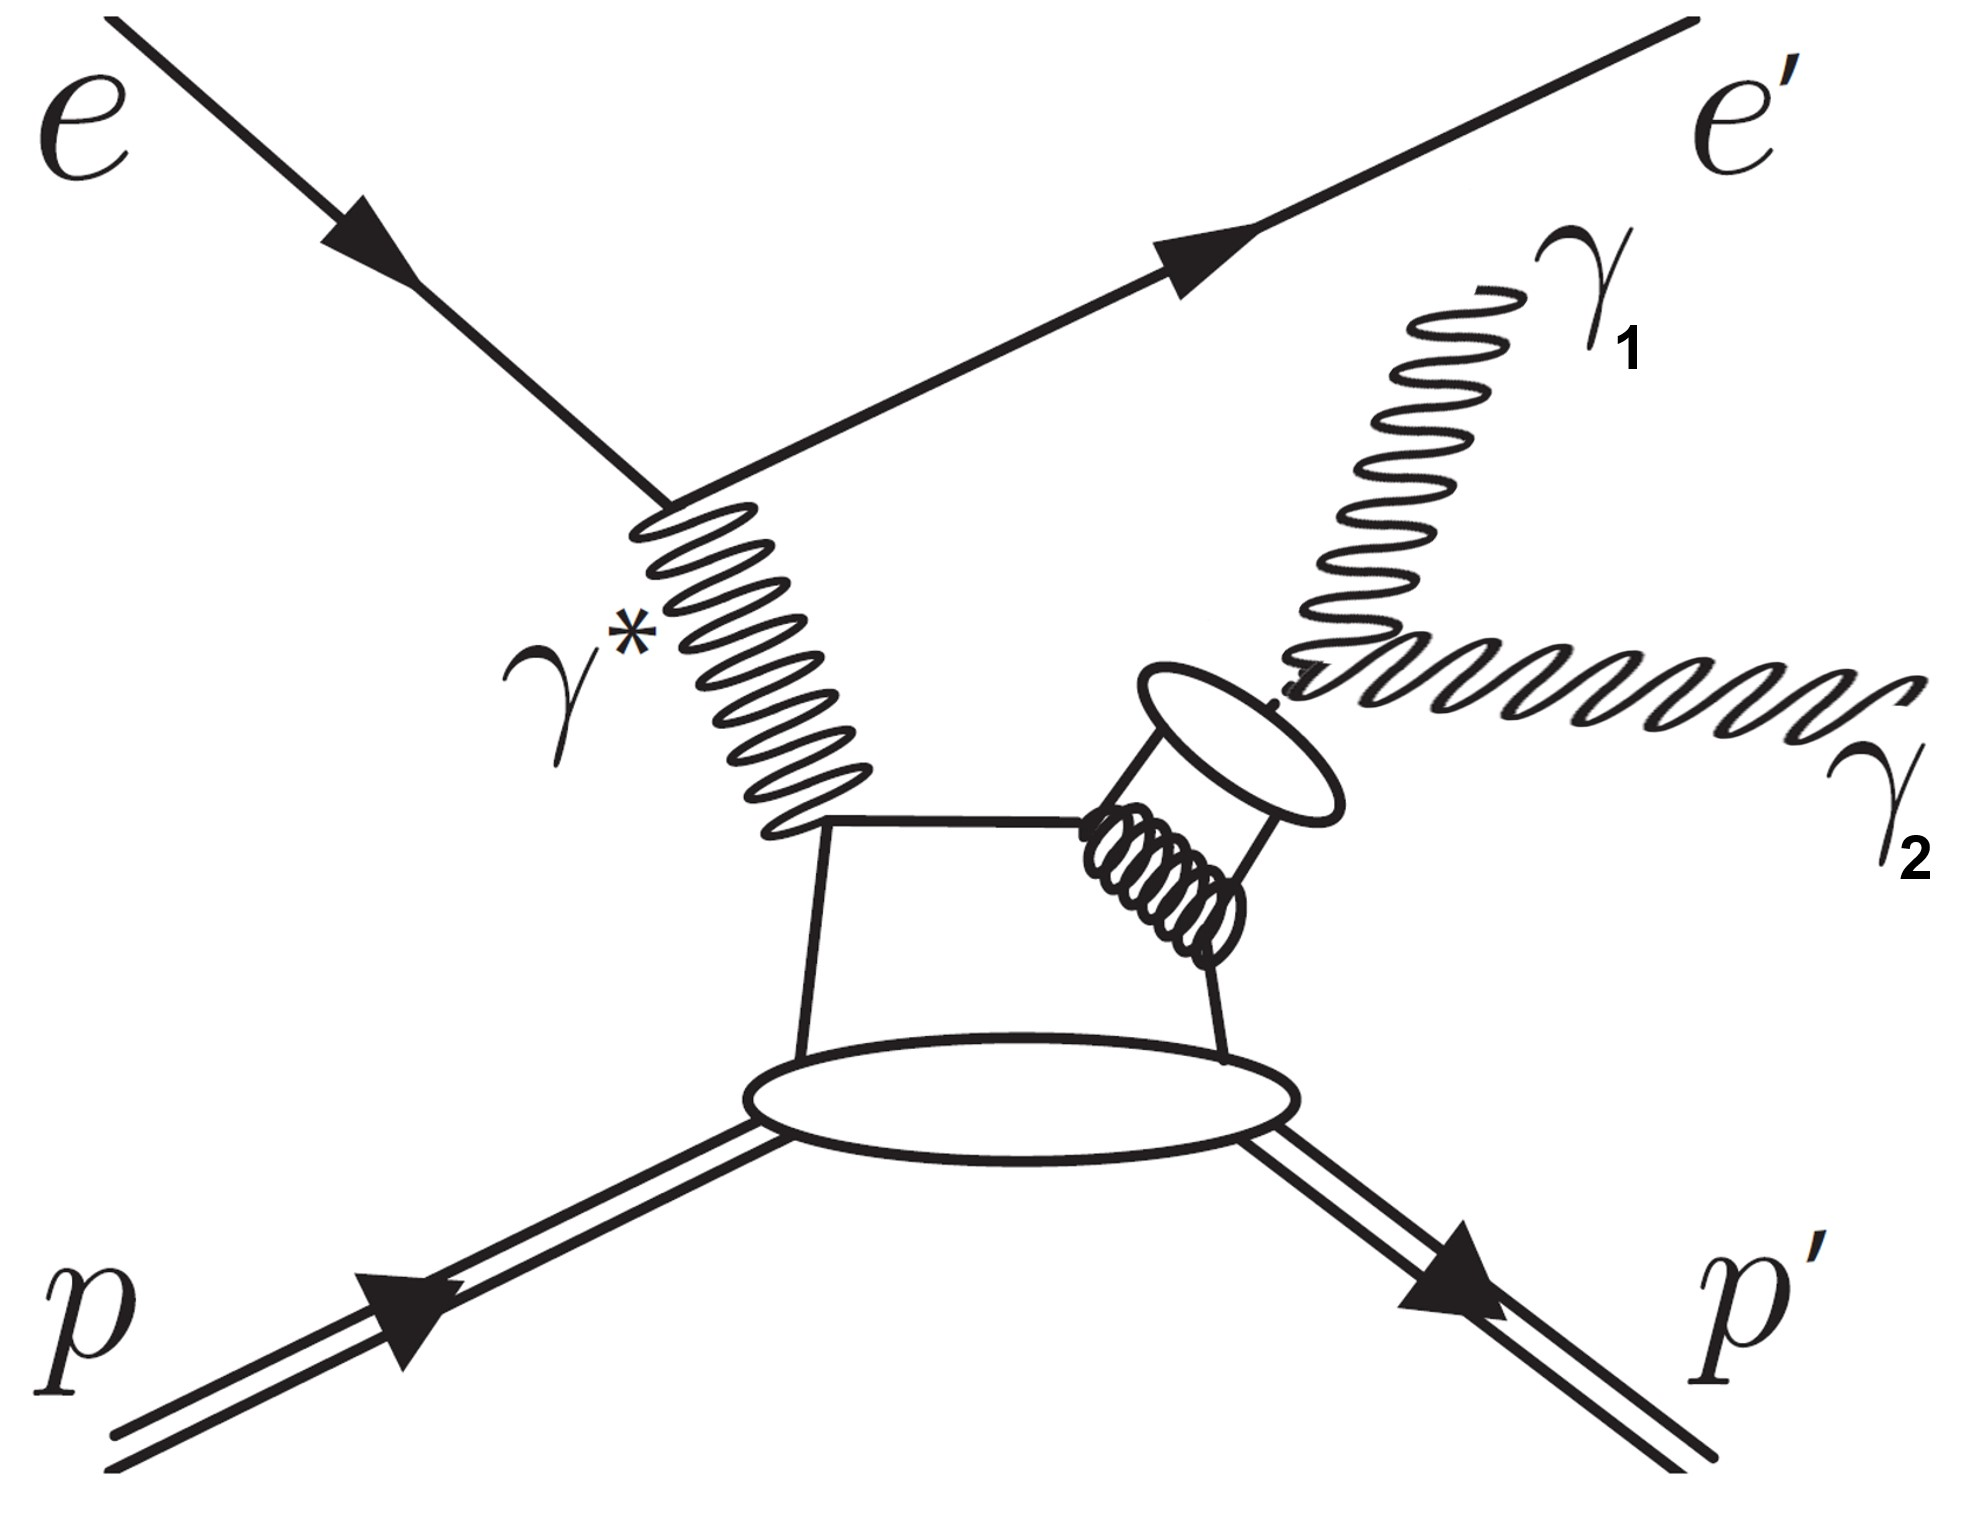
\includegraphics[width=0.5\textwidth]{Chapters/Ch1-Intro/Ch1-Sec2-GPDs-DVMP/pics/dvPiP_Feynman_diagram_2.jpg}
                \caption[DVPiP Feynman Diagram]{DV$\pi^0$P Feynman Diagram.}
                \label{fig:DVPiP_diagram}
            \end{figure}

            The unpolarized four-fold differential \xsec for DV$\pi^0$P can be decomposed into longitudinal and transverse structure functions as in \eqref{eq:DVPiPCrossSection_theory}, the formalism for which is covered in \parencite{Donnachie1978GeneralizedDominance}, \parencite{Dreschsel1992ThresholdNucleons}, and \parencite{Donnelly2023GeneralResponses}. 
            
            \iffalse
            \begin{equation}\labelAndRemember{eq:DVPiPCrossSection_theory}
                   {\frac{d^4\sigma_{ep \rightarrow ep'\pi^0}}{dQ^2dx_Bdtd\phi_{\pi}} =
                 \Gamma (Q^2, x_B, E)
                 \frac{1}{2\pi}
                 \left\{ \left(  \textcolor{sigmaT}{\frac{d\sigma_T}{dt}}+\epsilon  \textcolor{sigmaL}{\frac{d\sigma_L}{dt}} \right)+
                 \epsilon cos(2\phi)  \textcolor{sigmaTT}{\frac{d\sigma_{TT}}{dt}} + 
                 \sqrt{2\epsilon(1+\epsilon)} cos(\phi)  \textcolor{sigmaLT}{\frac{d\sigma_{LT}}{dt}} \right\}}.
             \end{equation}     
             \fi
             
             \begin{equation}\labelAndRemember{eq:DVPiPCrossSection_theory}
                {\begin{split}
                \frac{d^4\sigma_{ep \rightarrow ep'\pi^0}}{dQ^2dx_Bdtd\phi_{\pi}} &=
                \Gamma (Q^2, x_B, E) \frac{1}{2\pi} \left\{ \left(  \frac{d\sigma_T}{dt}+\epsilon  \frac{d\sigma_L}{dt} \right) \right. \\
                &\left. + \epsilon \cos(2\phi)  \textcolor{sigmaTT}{\frac{d\sigma_{TT}}{dt}} + 
                \sqrt{2\epsilon(1+\epsilon)} \cos(\phi)  \textcolor{sigmaLT}{\frac{d\sigma_{LT}}{dt}} \right\}.
                \end{split}}
            \end{equation}    \myequations{  DV$\pi^0$P Cross Section Decomposition}

             Here $\Gamma$ is the virtual photon flux as in \eqref{eq:virtualphotonflux} and represents the number of virtual photons per scattered electron \parencite{Amaldi1979Pion-electroproduction}, $\epsilon$ is the ratio of transverse to longitudinally polarized photons \eqref{eq:virtualphotonpolarization}, $\phi$ is the angle between the lepton and hadron planes, as illustrated in \figref{fig:phi_trento} and given by \eqref{eq:phitrento}, t is the momentum transfer to the proton \eqref{eq:t_momentum_trans}, $x_B$ and Q$^2$ are as given in \eqref{eq:xB} and \eqref{eq:virtualphotonflux} respectively, and the structure functions can be expressed as convolutions of GPDs as shown in \eqrange{eq:sigmaL}{eq:sigmaTT} as discussed in \parencite{Bedlinskiy2014ExclusiveCLAS}. 
  
    
            \begin{equation}\label{eq:virtualphotonflux}
                         \Gamma (Q^2, x_B, E) = \frac{\alpha}{8\pi} \frac{Q^2}{m^2_pE^2}\frac{1-x_B}{x_B^3}\frac{1}{1-\epsilon}
            \end{equation}\myequations{ Virtual Photon Flux}
        
            \begin{equation}\label{eq:virtualphotonpolarization}
                \epsilon = \frac{1 - y - \frac{Q^2}{4E^2}}{1 - y + \frac{y^2}{2} + \frac{Q^2}{4E^2}}
            \end{equation}\myequations{Virtual Photon Polarization}

            \begin{equation}\label{eq:phitrento}
                \phi = \cos^{-1} \left( \frac{ \left(p_{e} \times p_{e'} \right) \cdot \left( p_{p'} \times p_{\gamma^*} \right) }{ \lVert p_{e} \times p_{e'} \rVert \: \lVert p_{p'} \times p_{\gamma^*} \rVert} \right)
            \end{equation}\myequations{Lepton-Hadron Angle $\phi$}

            \begin{equation}\label{eq:t_momentum_trans}
                -t = -(p_{p'}-p_p)^2
            \end{equation}\myequations{Momentum Transfer t}


            \begin{figure}[H]
                \centering
                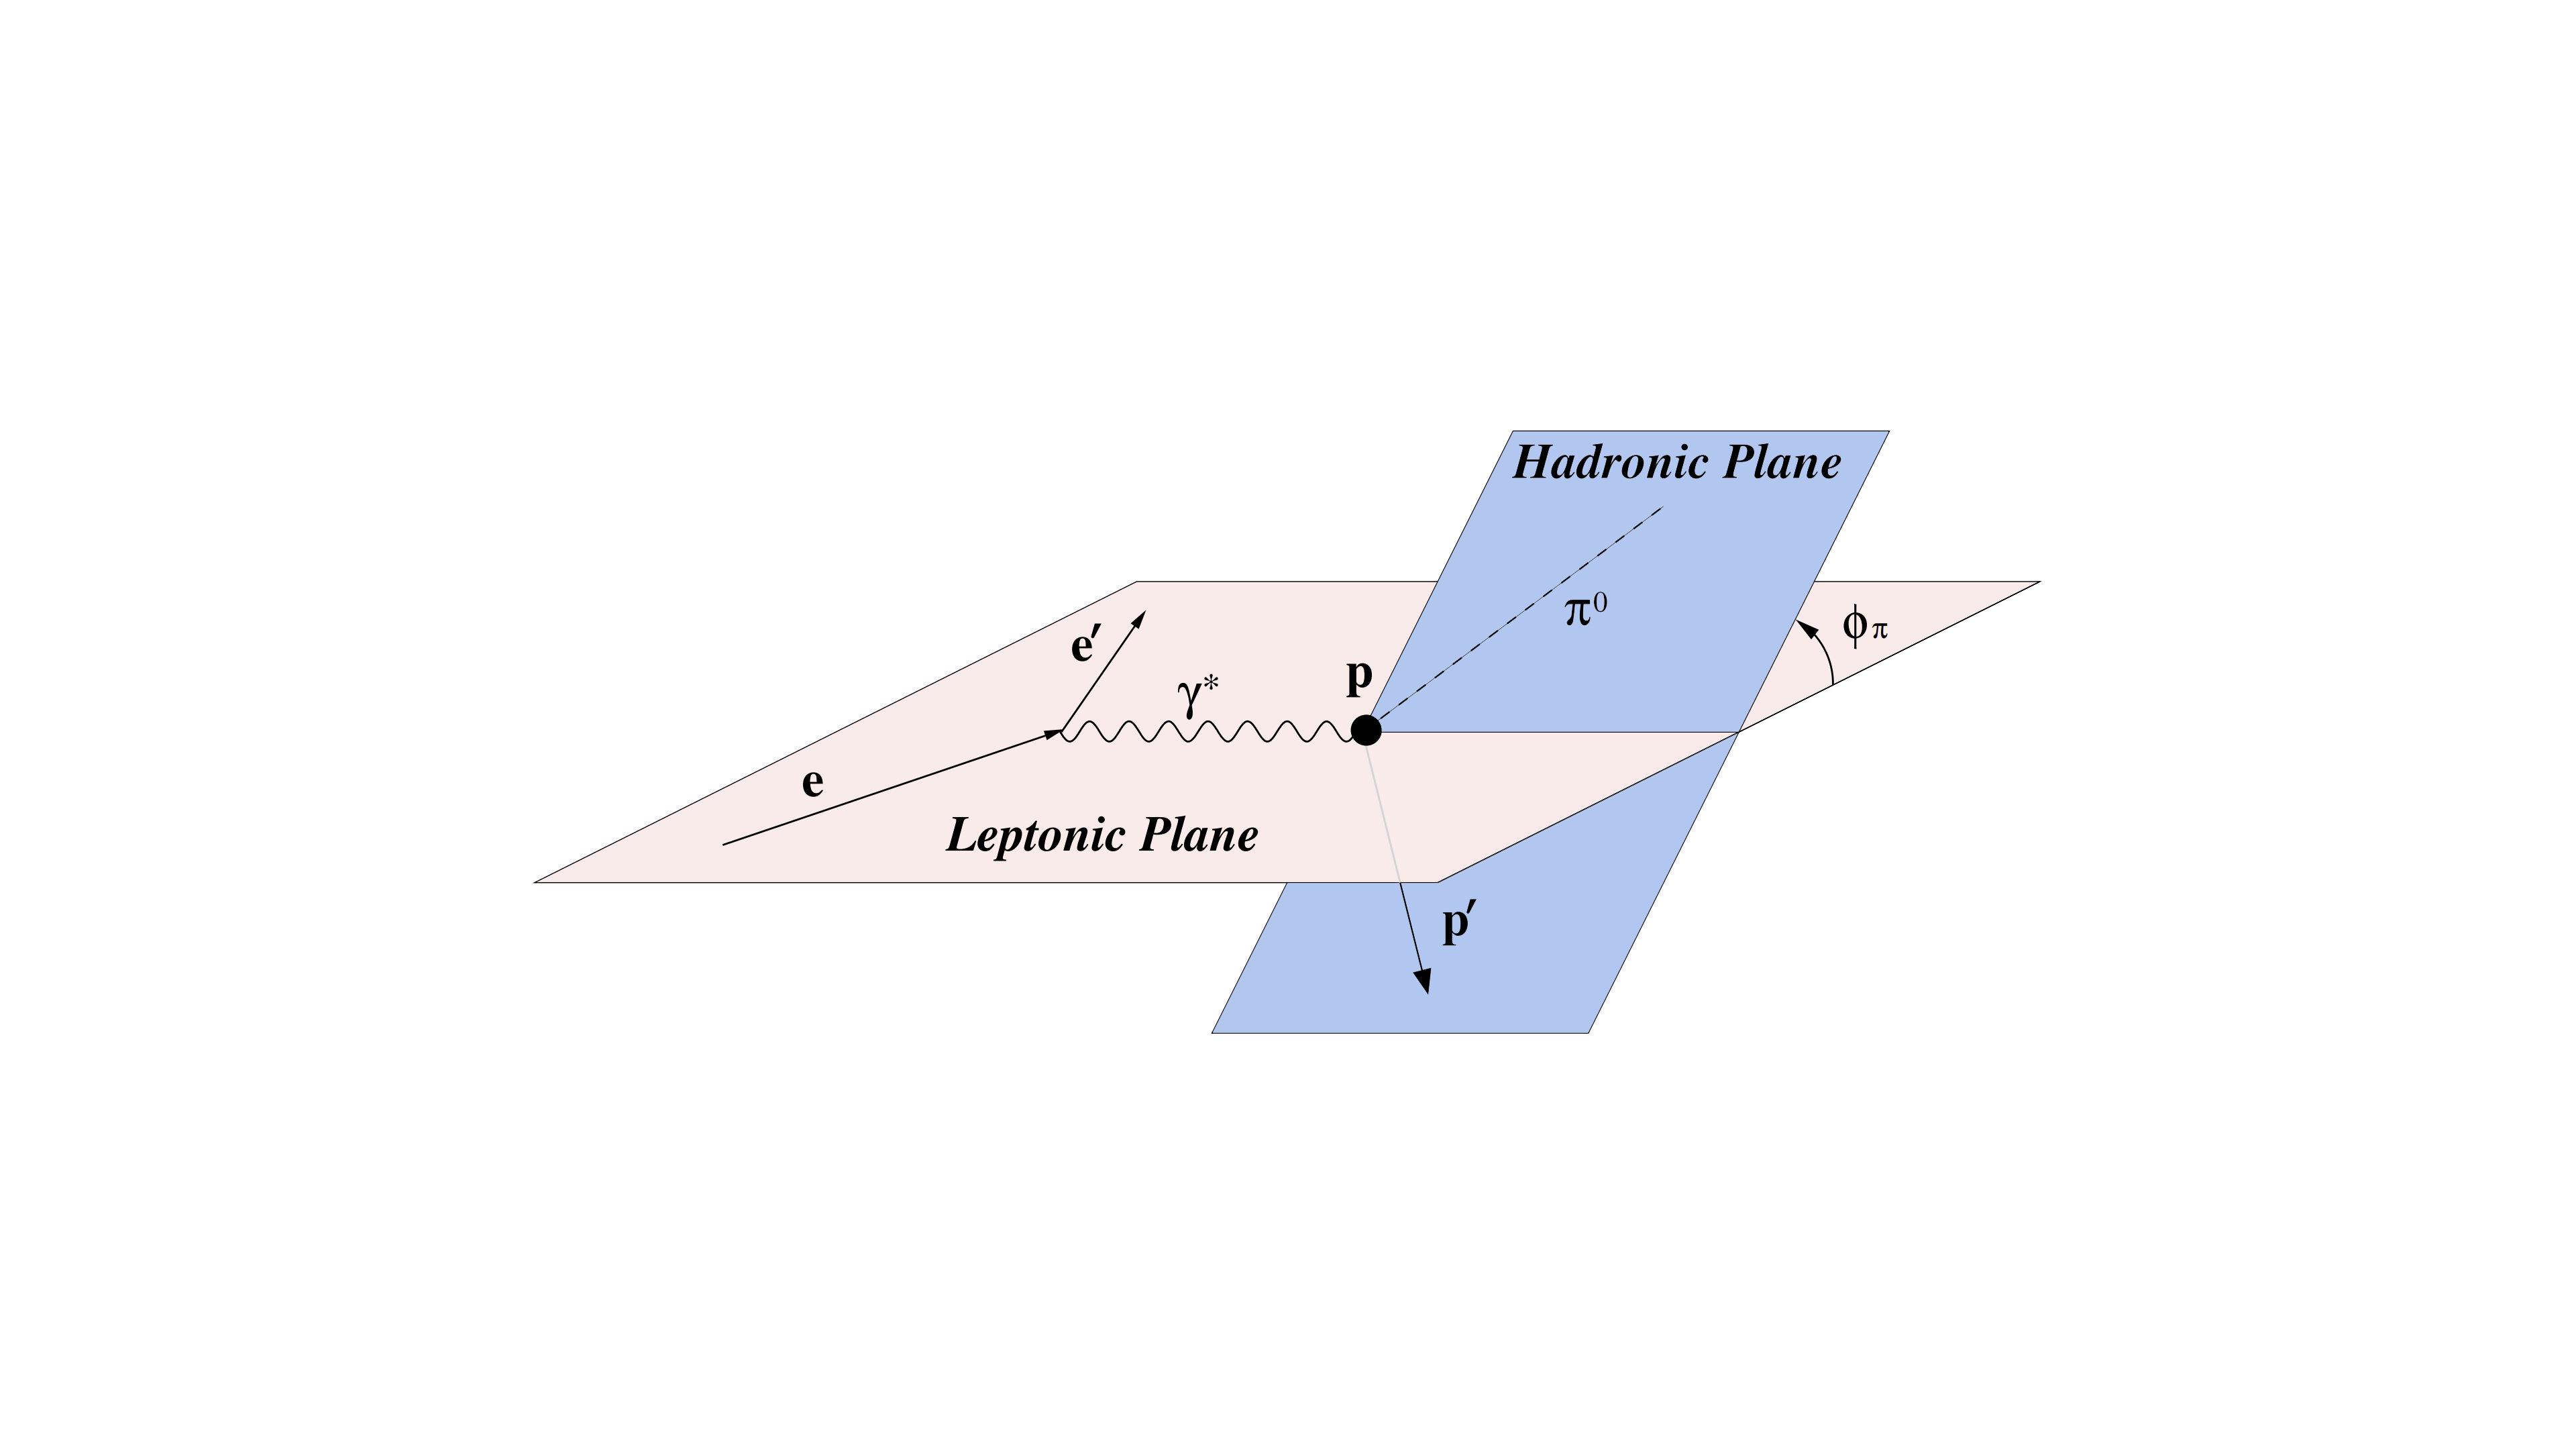
\includegraphics[width=0.99\textwidth]{Chapters/Ch1-Intro/Ch1-Sec2-GPDs-DVMP/pics/lept_had_planes.png}
                \caption{Diagram of Lepton-Hadron Plane Angle $\phi$.}
                \label{fig:phi_trento}
            \end{figure}

        
        
         \begin{equation}\label{eq:sigmaL}
                 \textcolor{sigmaL}{\frac{d\sigma_{L}}{dt}} = 
                \frac{4\pi\alpha}{kQ^2}\left\{ \left( 1 - \xi^2 \right) 
                \lvert \langle \GPDHtildeEQ \rangle \rvert ^2 
                -2\xi^2 \Re \left[  \langle \GPDHtildeEQ \rangle ^* \langle \GPDEtildeEQ \rangle    \right] - \frac{t'}{4m^2}\xi^2
                \lvert \langle \GPDEtildeEQ \rangle \rvert ^2  \right\}
            \end{equation} 
        
            \begin{equation}\label{eq:sigmaT}
                \textcolor{sigmaT}{\frac{d\sigma_{T}}{dt}} = 
                \frac{2\pi\alpha \mu_{\pi}^2}{kQ^4}
                \left\{ \left( 1 - \xi^2 \right) 
                \lvert \langle \GPDHTEQ \rangle \rvert ^2
                - \frac{t'}{8m^2}
                \lvert \langle \GPDETbarEQ \rangle \rvert ^2  \right\}    
            \end{equation} 
            
            \begin{equation}\label{eq:sigmaLT}
                \textcolor{sigmaLT}{\frac{d\sigma_{LT}}{dt}} = 
                \frac{4\pi\alpha \mu_{\pi}}{\sqrt{2}kQ^3}
                \xi\sqrt{1-\xi^2}
                \frac{\sqrt{-t'}}{2m}
                \Re \left\{ 
                 \langle \GPDHTEQ \rangle ^*
                \langle \GPDEtildeEQ \rangle   
                \right\}
             \end{equation} 
            
            
            \begin{equation}\label{eq:sigmaTT}
                \textcolor{sigmaTT}{\frac{d\sigma_{TT}}{dt}} = 
                \frac{4\pi\alpha \mu_{\pi}^2}{kQ^4}
                \frac{-t'}{16m^2}
                \langle \GPDETbarEQ \rangle^2   
            \end{equation} 
        
        
    
            The terms involved in these expressions are:
           
            \begin{itemize}
            \item t' = t - $t_0$ where $t_0 = \frac{-4m^2\xi^2}{1-\xi^2}$
            \item Skewness $\xi = \frac{x_B}{2-x_B}$
            \item   The bracket $\langle \tilde{F} \rangle$ is the convolution of a GPD and an appropriate subprocess amplitude:
            $
            \langle \tilde{F} \rangle =  \Sigma_{\lambda} \int_{-1}^{1} d\bar{x}H_{0\lambda,0\lambda}\left( \bar{x}, \xi, Q^2, t=0  \right)\tilde{F}\left( \bar{x}, \xi, Q^2, t  \right)\  
            $
            \begin{itemize}
                \item $\lambda$ is the unobserved helicites of the partons participating in the subprocess 
            \end{itemize}
            \item Phase space factor \scalebox{1}{%
             $           k = 16\pi \left( W^2 -m^2)\sqrt{\Lambda(W^2,-Q^2,m^2)} \right)$ 
            }
            \begin{itemize}
            \item $\Lambda(W^2,-Q^2,m^2)$ is the Källén function: $W^4 + Q^4 + m^4 + 2W^2Q^2 + 2Q^2m^2 - 2W^2m^2$
            \end{itemize}
            
            \item Scale parameter    \scalebox{1}{%
              $         \mu_{\pi^0} = \frac{m^2_{\pi^0}}{m_u+m_d}$ 
            }
            \begin{itemize}
                \item   $m_u$ and $m_d$ are respective masses of up and down quarks using the $\bar{MS}$ renormalization scheme. \parencite{Goloskokov2010AnElectroproduction}.
            \end{itemize}
            \end{itemize}
       
    %\subsection[Status of DVPiP Measurements]{Status of DV$\pi^0$P Measurements}
    
    \subsection{Status of DV\texorpdfstring{$\pi^0$}{pi0}P Measurements}


        With theoretical advancements occuring in the mid 1990s to early 2000s, the first analyses of experimental measurements of \dvpip have only been released in the past decade.
              
        \subsubsection*{Summary of Existing Measurements}

         The earliest of such measurements were take at the Thomas Jefferson National Accelerator Facility (JLab) with a $\sim$ 6 GeV electron beam. Two of the four experimental halls - Hall A \parencite{Fuchey2011ExclusiveRegime} and Hall B \parencite{Bedlinskiy2014ExclusiveCLAS} produced \xsec results. Hall A houses a small acceptance precision spectrometer and recorded data in several kinematic bins. Hall B housed a large acceptance spectrometer, yielding \xsec measurements over a large kinematic regime. 
         %Hall A Rosenbluth separation \parencite{Defurne2016RosenbluthSection}
         
         Recent upgrades at JLab have nearly doubled the beam energy to 10.6 GeV, and both detector halls have accumulated data allowing for the measurement of this process. Both halls repeated data taking at this higher energy, with Hall A recently releasing updated \xsec values across three fixed $x_B$ bins (0.36,0.48 and 0.6) and over a range of $Q^2$ values from 3 to 9 GeV$^2$ \parencite{Dlamini2021DeepRegime}. 
         
         This work expands on these results by covering a much larger kinematic regime, as well as having much higher statistics compared to the 6 GeV Hall B result. A kinematic overlap plot in $Q^2$, $x_B$ is shown in \figref{fig:kinematicreach} summarizes these differences. It is also noted that the CERN COMPASS collaboration \parencite{Alexeev2020MeasurementProton} has measured this process using a 160 GeV muon beam, obtaining results over a much lower $x_B$ range.  

       
         %However, for pi0 the only data we have from Hall A are of very limited statistics and kinematics. One of their limitations was the relatively modest variation on polarization parameter (epsilon) since the beam energies we not so far apart. 
    
     
        \begin{figure}[H]
            \centering
            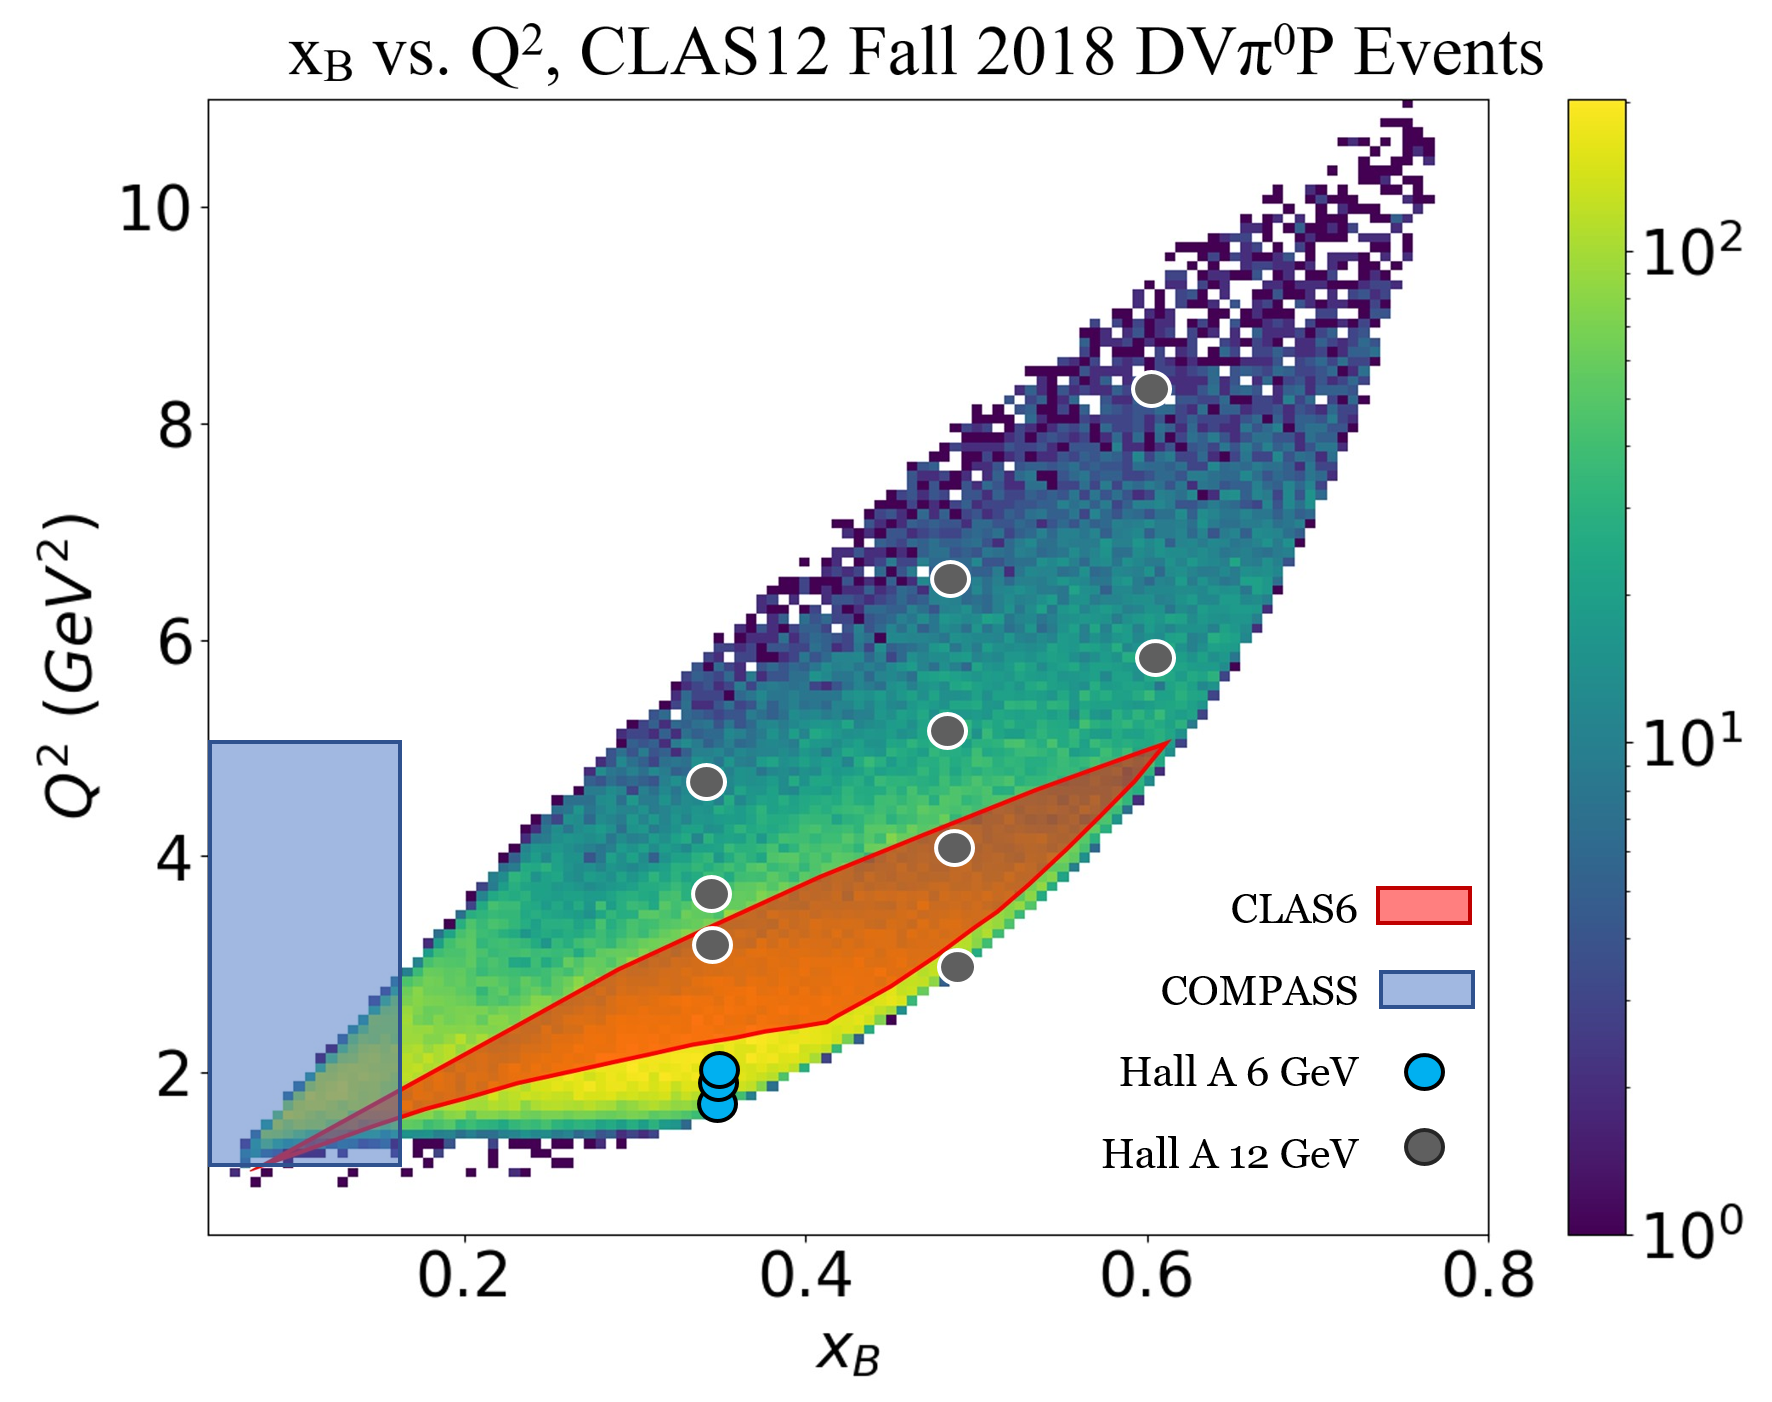
\includegraphics[width=0.75\textwidth]{Chapters/Ch1-Intro/Ch1-Sec2-GPDs-DVMP/pics/kinematic_overlap.png}
            \caption[Kinematic Reach Comparison]{Kinematic reach plot between this work and other results:  CLAS6 (red polygon) \parencite{Bedlinskiy2014ExclusiveCLAS}, COMPASSS (blue rectangle) \parencite{Alexeev2020MeasurementProton}, Hall A 6 GeV (blue dots) \parencite{Fuchey2011ExclusiveRegime}, and Hall A 12 GeV (gray dots) \parencite{Dlamini2021DeepRegime}, overlaid on the event data of this work (multicolored histogram). The reach shown for Hall A are approximate areas around their reported bin centers. }
            \label{fig:kinematicreach}
        \end{figure}

        \subsubsection*{Overview of This Analysis}\label{sec:anaflow}
    
    
        This work details the analysis of data taken at the JLab CLAS12 experiment to measure the deeply virtual neutral pion electroproduction \xsecp The general form of a scattering cross section, \eqref{eq:basic_diff_xsec} copied below, is true in the idealized case where all measurements are perfect. In practice, a number of correction terms need to be included to account for differences between experiment and theory. These correction terms, combined with the specifics of this analysis (four-fold differential \xsec), yield the full experimental expression of the \xsec \eqref{eq:DVPiPCrossSection_exp}. 


        \begin{equation*}
          \recallLabel{eq:basic_diff_xsec}
        \end{equation*}
  
       
             \begin{equation}\labelAndRemember{eq:DVPiPCrossSection_exp}
                   { \frac{    d^4\sigma_{  ep \rightarrow ep'\pi^0}   } {dQ^2dx_Bdtd\phi_{\pi}} 
                        =   \frac{ \textcolor{red}{ N(Q^2,x_B,t,\phi_{\pi})}} {\Lumiint \textcolor{purple}{ \Delta Q^2 \Delta x_B \Delta t \Delta \phi_{\pi}}} 
                        \frac{1}{\textcolor{correctionfactors}{\epsilon_{acc} \delta_{RC} \delta_{Norm} Br(\pi^0\rightarrow\gamma\gamma)}}}
             \end{equation}      \myequations{DV$\pi$P Experimental Cross Section}
        
        The terms on the right-hand side of this equation are: 
        \begin{itemize}
        \item \textcolor{red}{$N(Q^2,x_B,t,\phi_{\pi})$} - Number of events recorded in a given $Q^2$, $x_B$, $t$, $\phi_{\pi}$ bin.
        
        \item \Lumiint - Integrated luminosity
        
        \item \textcolor{purple}{$\Delta Q^2 \Delta x_B \Delta t \Delta \phi_{\pi}$} - These are the bin sizes or intervals for the variables $Q^2$, $x_B$, $t$, and $\phi_{\pi}$.
        
        \item \textcolor{correctionfactors}{$\epsilon_{acc}$} - Acceptance correction, which is a combination of detector efficiency and geometrical acceptance, determined through simulations. 
        
        \item \textcolor{correctionfactors}{$\delta_{RC}$} - Radiative correction factor
        
        \item \textcolor{correctionfactors}{$\delta_{Norm}$} - Overall normalization factor
        
        \item \textcolor{correctionfactors}{$Br(\pi^0\rightarrow\gamma\gamma)$} - Branching ratio of the decay of a neutral pion ($\pi^0$) into two photons ($\gamma\gamma$), which is most recently measured at 98.8131\%  \parencite{Husek2019PreciseDecay}
        \end{itemize}

        The numerous correction factors motivate approaching this analysis in terms of an \textit{inverse problem}. This class of inference problems requires using data and statistical methods to provide a best estimate of an unknown underlying event or distribution, given a set of observables produced by that unknown generator. To realize a high quality estimate of the underlying physics processes (GPDs) we measure the observables of that process - DVEP event rates - as discussed in Chapter \ref{Chapter:Experiment}. We also produce simulated observables through physics generators and event simulators as covered in Chapter \ref{Chapter:Simulations}. Chapter \ref{Chapter:BaseAnalysis} compares the generated, simulated, and experimental data, which allows for inference of the underlying physics - a \xsec measurement with proper correction terms. Chapter \ref{Chapter:Ch5_IBU} discusses statistical methods to improve on a bin-by-bin analysis. Finally, Chapter \ref{Chapter:Further Analysis} then presents further physics analysis, made possible with the extracted \xsec values. \figref{fig:ProcessFlowchart} broadly summarizes the analysis flow; electronic readers can conveniently click on boxes for hyperlinks to relevant sections. 

        %discusses the computational and simulational infrastructure built and used as an integral part in estimating correction factors and performing an accurate measurement. 


            \begin{figure}
                \centering
                  \resizebox{15.cm}{!}{\begin{tikzpicture}[
                    node distance=1cm,
                    box/.style={rectangle, rounded corners, draw=black, thick, minimum width=5cm, minimum height=.9cm, align=center},
                    bigbox/.style={rectangle, rounded corners, draw=black, thick, minimum width=10.5cm, minimum height=1cm, align=center},
                    biggestbox/.style={rectangle, rounded corners, draw=black, thick, minimum width=16cm, minimum height=1cm, align=center}
                ]
            
            
                % First column
                \node[box, fill=blue!30] (c1b1) {\hyperref[sec:ch1sec2GPDs]{Underlying Physics}};
                \node[box, fill=blue!30, below=of c1b1] (c1b2)  {\hyperref[sec:clas12exp]{CLAS12 Experiment}};
                \node[box, fill=blue!30, below=of c1b2] (c1b3)  {\footnotesize Experimental Detector Signals};
                \node[bigbox, fill=orange!30, below=of c1b3, xshift=2.75cm] (c1b4)  {\hyperref[sec:decoding_reconstruction]{Decoding and Reconstruction}};
                \node[bigbox, fill=orange!30, below=of c1b4] (c1b5)  {\hyperref[sec:filtering]{Fiducial Filtering and File Conversion}};
                \node[box, fill=orange!30, below=of c1b5,  xshift=-2.75cm] (c1b6) {\hyperref[sec:momcorr]{Momentum Corrections}};
                \node[bigbox, fill=orange!30, below=of c1b6, xshift=2.75cm] (c1b7)  {\hyperref[sec:Ch4_event_selection]{Event Selection}};
                \node[box, fill=blue!30, below=of c1b7,  xshift=-2.75cm] (c1b8) {Experimental Events};
                
                % Second column
                
                \node[box, fill=red!30, right=.5cm of c1b2] (c2b2) {\hyperref[sec:sim_pipeline] {\footnotesize GEANT4 Simulation}};
                \node[box, fill=red!30, below=of c2b2] (c2b3) {\footnotesize Simulated Detector Signals};
                \node[box, fill=orange!30, right=0.5cm of c1b6] (c2b6) {\hyperref[sec:momsmear]{Momentum Smearing}};
                \node[box, fill=red!30,  right=0.5cm of c1b8] (c2b8) {Simulated Events};
            
                % Third column
                \node[box, fill=green!30, right=6cm of c1b1] (c3b1) {\hyperref[sec:ch3generator] {\footnotesize Computational Event Generator}};
                \node[box, fill=green!30, right=6cm of c1b8] (c3b4) {Generated Events};
            
                % Combined final column
                \node[biggestbox, fill=blue!30, below=of c2b8] (ccb9) {\hyperref[Chapter:BaseAnalysis]{\Xsec Measurement}};
    
                \node[biggestbox, fill=blue!30, below=of ccb9] (ccb10) {\hyperref[Chapter:Further Analysis]{Further Analysis}};
                
                
                % Arrows for first column
                \draw[->] (c1b1) -- (c1b2);
                \draw[->] (c1b2) -- (c1b3);
                \draw[->] ([xshift=0cm]c1b3.south) -- ([xshift=0cm]c1b3.south |- c1b4.north);
                 
                \draw[->] (c1b4) -- (c1b5);
                \draw[->] ([xshift=0cm]c1b6.north |- c1b5.south) -- ([xshift=0cm]c1b6.north);
                \draw[->] ([xshift=0cm]c1b6.south) -- ([xshift=0cm]c1b6.south |- c1b7.north);
                \draw[->] ([xshift=0cm]c1b8.north |- c1b7.south) -- ([xshift=0cm]c1b8.north);
                
                % Arrows for second column
                \draw[->] (c2b2) -- (c2b3);
                \draw[->] ([xshift=0cm]c2b3.south) -- ([xshift=0cm]c2b3.south |- c1b4.north);
                \draw[->] ([xshift=0cm]c2b6.north |- c1b5.south) -- ([xshift=0cm]c2b6.north);
                \draw[->] ([xshift=0cm]c2b6.south) -- ([xshift=0cm]c2b6.south |- c1b7.north);
                \draw[->] ([xshift=0cm]c2b8.north |- c1b7.south) -- ([xshift=0cm]c2b8.north);
                
                
                % Arrows for third column
                \draw[->] (c3b1) -- (c3b4);
                \draw[->] (c3b1) -- (c2b2);
            
                \draw[->] (c3b4) -- (ccb9);
                \draw[->] (c1b8) -- (ccb9);
                \draw[->] (c2b8) -- (ccb9);
    
    
                \draw[->] (ccb9) -- (ccb10);    
                
                \end{tikzpicture}}
                \caption[Analysis Flowchart]{Analysis Overview Flowchart.}
                \label{fig:ProcessFlowchart}
            
            \end{figure}
    
   
    \iffalse
    \section{extra}
    
                      Only valence quarks contribute electroproduction of uncharged pions.
               
            Several weeks ago I remarked in our meeting that I was having difficulty finding an explanation for the specific form of the DVMP cross section written in terms of structure functions (example below). Papers normally state that the relation holds without justification. I tried to follow the papertrail for the origin but so far have not ultimately been successful. Igor has kindly found a paper from 1992 (Dreschsel and Tiator pdf (iop.org) which makes reference (page 460, eq 18 - 19) \parencite{Dreschsel1992ThresholdNucleons}
            \parencite{Bedlinskiy2014ExclusiveCLAS} to Donnachie and Shaw (Generalized Vector Dominance 1978) \parencite{Donnachie1978GeneralizedDominance}
            
            
            In the attached, Bill Donnelly and colleagues have recently published a long paper
            on the general tensor structure for electron scattering in terms of invariant responses.
            In Eq (46), they derive a general expression for the Lorentz invariant part of the spin \parencite{Donnelly2023GeneralResponses}
            dependent cross section.  The unpolarized piece has the identical L/T/TT/TL form you have.
            I have not read the paper in detail but I think you may find it useful.


            
            Here is a quote from their intro.
            "... deeply virtual $\pi^0$ (as well as $\eta$, $\eta'$) production off a proton target is clearly distinct from the other types of meson production processes in that it involves the transition of a (virtual) photon with JPC = 1-- to a JPC = 0-+ state (i.e. the final $\pi^0$ or $\eta$, $\eta$') requiring odd C-parity and chiral odd t-channel quantum numbers. As a consequence, in a partonic description such as the one depicted in Fig.1a, the ”outgoing” and ”returning” quark helicities need to be opposite to one another …". 

    
        	However,  since the pi0 and eta are JP=0-, then the transverse photon part contributing to the overall reaction cross section can cause a transversely polarized  quark helicity flip. This is contained mainly  in the structure functions $\sigma_T$ and $\sigma_{TT}$, which can be decomposed into the transverity GPDs - mainly $Ebar_T$ and $H_T$. 
        	
        	Also, pion and eta production can still also be accompanied by non-quark helicity flips, which would be mainly contained in the longitudinal structure functions $\sigma_{LL}$. However, various theoretical papers indicate that in our accessible region of $Q^2$, $\sigma_T$ and $\sigma_{TT}$ dominate relative to $\sigma_L$. Experimentally, this seems to be verified from JLab data .
        	On the other hand, theory predicts that asymptotically, $\sigma_L$ will dominate. From our existing 5 GeV  data, we are not anywhere near there, so our experiments at JLab are really just right for accessing these transversity distributions.  But, to decompose these distributions  at the level of the individual quark u d flavors, we need as much precision data over as big a range as possible of kinematics in several channels - P-pi0, N-pi0, P-eta, N-eta. And, only you guys can do that!
        	So, let me know if this makes sense to you. s a bit. 
        	
            If you look at the proposal you will see the main diagram we are interested in has a pair of gluons from the GPD bag connecting a the hard scattering kernel that comes from the virtual photon fluctuating into a $s\bar{s}$ pair
            
            The process you mention instead has a pair of strange quarks from the GPD bag connecting to the hard scattering kernel directly. 
            
            In practice the two processes happen. From known PDF however the gluon contribution is expected to be significantly larger than the strange quarks contribution. So the intuitive reason would be: the proton has nearly no strangeness but does have a bunch of gluons.
            
            Now it could be that we are wrong and that the proton has more strangeness than what conventional PDF suggest. This could potentially hamper our strategy. However, intrinsic strangeness is in itself a very interesting subject, and if we did come to the conclusion that the proton has more strangeness than is conventionally accepted, then it would be a very important result.
            
            The way I understand why the phi channel probes the gluon GPDs is because the phi meson is a strange-antistrange meson, and so doesn't interact with the up and down quarks that predominantly make up the quark content of the nucleons. This is from the phi cross section proposal: Because of its almost pure $s\bar{s}$ composition $\phi$ production is not affected by scattering from the nucleon’s valence quarks or the light quark sea;
            
                    virtual $\pi^0$ (as well as$\eta$,$\eta$') production off a proton target is clearly distinct from the other
            types of meson production processes in that it involves the transition of a (virtual) photon
            with JPC = 1– to a JPC = 0-+ state (i.e. the final $\pi^0$ or$\eta$,$\eta$’) requiring odd C-parity and
            chiral odd t-channel quantum numbers
For example, the phi, on which F-X and Patrick are
            working, is very sensitive to the gluon distribution in the nucleon.
herefore DVCS is
            primarily sensitive to non-quark spin flip - eg. H.. The same is true with DVMP of other
            vector meson, such as rho. However, since the pi0 and eta are JP=0-, then the transverse
            photon part contributing to the overall reaction cross section can cause a transversely po-
            larized quark helicity flip. This is contained mainly in the structure functions $\sigma$T and $\sigma$T T ,
            which can be decomposed into the transverity GPDs - mainly EbarT and HT


      By measuring DVMP, we can get information about GPDs in the following way: in the leading twist approximation / some other formalism bullshit, dvmp cross section is described by the generalized Compton form factors, which themselves are (to leading twist etc.) convolutions of GPDs, so the dvmp cross section sets constraints on GPD behavior. Hard exclusive pseudoscalar meson electroproduction in recent years has shown that the asymptotic leading twist approximation is not readily applicable in the range of kinematics accessible to current experiments. In fact, there are strong contributions from transversely polarized virtual photons that are asymptotically supprsed by $1/@^w$ in the cross sections and have to be considered by introduing chiral-odd GPDs into the framework.   
        
        So Q2>1 is indeed for deeply virtual events, however it has no relation with lepton/hadron angle. There are pi0 events in the region below 1GeV2, and they are also pi0 events. The limit on 1GeV2 is somewhat artificial. Ideally we are looking at the asymptotic freedom, so Q2 should be infinity, but we are hoping that 1GeV2 is big enough to apply models that are based on asymptotic freedom. There are many terms also that are proportional to powers of t/Q2. So we need reasonably big Q2 to apply GPDs models. And in fact CLAS kinematics is often questioned to be too small for GPDs theoretical models.
        
        DVMP is sensitive to chiral odd GPDs, distinguishing it from DVCS as a GDP probe because why? Because something involving photon helicity and pion helicity, I forget exactly though


            In DVCS the  incident and  outgoing particles are both photons JP= 1-. Therefore, no quark helicity flip is necessary in this “virtual Compton scattering”.  Therefore DVCS is primarily sensitive to non-quark spin flip - eg. H.. The same is true with DVMP of other vector meson, such as rho.
            
    
            First, note that not all DVMP reactions are sensitive to nuclear transversity distributions, which involves quark helicity flip of transversely polarized quarks helicity  This can occur in  production of pseudoscaler mesons,  e.g. pi0 and eta production, with spin-charge-parity  I-PC= 0 - + ,in contrast with  the incident photon, which  has J-P 1- -. 
            
            This is not the case for other mesons studied at JLab, such as vector mesons, I-PC= 0 - e.g. the rho, omega, phi, for which which I-CP= 1- -, the same as for the photons.   
            
            I believe this was first  pointed out  Ahmad, Goldstein, Liutti (arXiv:0805.3568). 

            
            
    \fi
    
%%%%%%%%%%%%%%%%%%%%%%%%%%%%%%%%%%%%%%%%%%%%%%%%%%%%%%%%%%%%%%%%%%%%%%%%%%%%%%%%%%%%%%%%%%%%%%%%%%%%%%%%%%%%%%%%%%%%%%%%%%%%%%%%%%%%%%%%%%%%%%%%%%%
%%%%%%%%%%%%%%%%%%%%%%%%%%%%%%%%%%%%%%%%%%%%%%%%%%%%%%%%%%%%%%%%%%%%%%%%%%%%%%%%%%%%%%%%%%%%%%%%%%%%%%%%%%%%%%%%%%%%%%%%%%%%%%%%%%%%%%%%%%%%%%%%%%%
%%%%%%%%%%%%%%%%%%%%%%%%%%%%%%%%%%%%                 EXTRA STUFF                                                        %%%%%%%%%%%%%%%%%%%%%%%%%%%
%%%%%%%%%%%%%%%%%%%%%%%%%%%%%%%%%%%%%%%%%%%%%%%%%%%%%%%%%%%%%%%%%%%%%%%%%%%%%%%%%%%%%%%%%%%%%%%%%%%%%%%%%%%%%%%%%%%%%%%%%%%%%%%%%%%%%%%%%%%%%%%%%%%
%%%%%%%%%%%%%%%%%%%%%%%%%%%%%%%%%%%%%%%%%%%%%%%%%%%%%%%%%%%%%%%%%%%%%%%%%%%%%%%%%%%%%%%%%%%%%%%%%%%%%%%%%%%%%%%%%%%%%%%%%%%%%%%%%%%%%%%%%%%%%%%%%%%




\iffalse
\begin{tikzpicture}
    \begin{feynman}
        \vertex (i1) {$e^{-}$};
        \vertex[right=1cm of i1] (v1);
        \vertex[below=2cm of i1] (i2) {$p$};
        \vertex[right=1cm of i2] (v2);
        \vertex[right=2cm of v1] (o1) {$e^{-}$};
        \vertex[right=2cm of v2] (o2) {$p$};
        \vertex[above right=1cm and 1cm of v2] (v3);
        \vertex[right=1cm of v3] (o3) {$\bar{q}$};
        \vertex[below right=1cm and 1cm of v3] (o4) {$q$};

        \diagram* {
            (i1) -- [fermion] (v1) -- [fermion] (o1),
            (i2) -- [fermion] (v2) -- [fermion] (o2),
            (v1) -- [photon, edge label=$\gamma^{*}$] (v2),
            (v2) -- [fermion] (v3),
            (v3) -- [fermion] (o3),
            (v3) -- [anti fermion] (o4),
        };
    \end{feynman}
\end{tikzpicture}
\fi
    %Deeply (Q2 >> M^2) Inelastic (W2 >>M2) Scattering


\iffalse
Stuff to add sometime / for consideration:


        %     Ji discusses gauge-invariant spin in his 1997 study \parencite{Ji1997Gauge-InvariantSpin}.
         %   attempt to understand pion production \parencite{Goloskokov2010AnElectroproduction}
         %   Burkardt's 2007 work investigates Generalized Parton Distributions (GPDs) \parencite{Burkardt2007GPDs0}.
            

    

        In addition to collinear momentum distribution of partons inside the
        nucleon, GPDs also encode the distribution of partons in the plane transverse to
        the nucleons momentum in the infinite momentum frame [58]. Moreover, their
        relation to energy-momentum tensor (EMT) form factors allow us to access the
        EMT densities, the distribution of energy, angular momentum, pressure, and shear
        forces inside the nucleon     

        

              Jaffe deep physics \parencite{Jaffe2022DeepPhysics} 
            Goloskokov's 2011 work delves into transversity of mesons \parencite{Goloskokov2011TransversityMesons}.


            Intuition about DVMP
            First, note that not all DVMP reactions are sensitive to nuclear transversity distributions,
            which involves quark helicity flip of transversely polarized quarks helicity This can occur
            in production of pseudoscaler mesons, e.g. pi0 and eta production, with spin-charge-parity
            I-PC= 0 - + ,in contrast with the incident photon, which has J-P 1- -. This is not the case
            for other mesons studied at JLab, such as vector mesons, I-PC= 0 - e.g. the rho, omega, phi,
            for which which I-CP= 1- -, the same as for the photons. I believe this was first pointed out
            Ahmad, Goldstein, Liutti (arXiv:0805.3568). Here is a quote from their intro. ”... deeply
            virtual $\pi^0$ (as well as$\eta$,$\eta$') production off a proton target is clearly distinct from the other
            types of meson production processes in that it involves the transition of a (virtual) photon
            with JPC = 1– to a JPC = 0-+ state (i.e. the final $\pi^0$ or$\eta$,$\eta$’) requiring odd C-parity and
            chiral odd t-channel quantum numbers. As a consequence, in a partonic description such
            as the one depicted in Fig.1a, the ”outgoing” and ”returning” quark helicities need to be
            opposite to one another . . . ”.
            Peter Kroll, who works very closely this group, with Sergei Goloskokov, Marcus Diehl,
            et al. have published extensive theoretical calculations based on Jlab data. Gary Goldstein,
            Simonetta Liutti have have also published on this reaction.
            By the way, the other meson production channels are uniquely sensitive to other inter-
            esting aspects of nucleon structure. For example, the phi, on which F-X and Patrick are
            working, is very sensitive to the gluon distribution in the nucleon.
            In DVCS the incident and outgoing particles are both photons JP= 1-. Therefore, no
            quark helicity flip is necessary in this “virtual Compton scattering”. Therefore DVCS is
            primarily sensitive to non-quark spin flip - eg. H.. The same is true with DVMP of other
            vector meson, such as rho. However, since the pi0 and eta are JP=0-, then the transverse
            photon part contributing to the overall reaction cross section can cause a transversely po-
            larized quark helicity flip. This is contained mainly in the structure functions $\sigma$T and $\sigma$T T ,
            which can be decomposed into the transverity GPDs - mainly EbarT and HT
            
            Also, pion and eta production can still also be accompanied by non-quark helicity flips,
            which would be mainly contained in the longitudinal structure functions $\sigma$LL. However,
            various theoretical papers indicate that in our accessible region of Q2, $\sigma$T and $\sigma$T T dominate
            relative to $\sigma$L. Experimentally, this seems to be verified from JLab data . On the other
            hand, theory predicts that asymptotically, $\sigma$L will dominate. From our existing 5 GeV data,
            we are not anywhere near there, so our experiments at JLab are really just right for accessing
            these transversity distributions. But, to decompose these distributions at the level of the
            individual quark u d flavors, we need as much precision data over as big a range as possible
            of kinematics in several channels - P-pi0, N-pi0, P-eta, N-eta. And, only you guys can do
            that! So, let me know if this makes sense to you. s a bit.
                       
            
            Low t-data are very important for the meson exclusive physics. The GPD interpretation
            works only in the region -t/Q2¡1. From this point of view the central detector will not only
            increase the total statistics by a factor more than 2 but will add the valuable data with low
            t.
            However, for pi0 the only data we have from Hall A are of very limited statistics and
            kinematics. One of their limitations was the relatively modest variation on polarization
            parameter (epsilon) since the beam energies we not so far apart.
            Number of final events in CLAS6 DVMP? About 100K, maybe 200K.
            Dear Valery
            CLAS12 acceptances and resolutions are also superior to that of CLAS6. Main differences
            are: - RGK has outbending torus vs inbending CLAS6 data - the distance between the target
            and the PCal has increased, the FTCal extends to lower angles, and the gap between FTCal
            and PCal is much smaller than between IC and EC - proton polar angle was limited to 60
            deg in the e1dvcs dataset if my memory is correct
            Do you have on hands the number of exclusive pi0 events published for the CLAS6
            \xsecs? We need numbers to make the case to cook the RGK data
            Well over an order of magnitude more statistics at CLAS12 compared to CLAS6


            In conclusion, it is important to place the discussion here in the context of a broader theoretical framework. Partons inside the proton can be described by Wigner distributions in six-dimensions (three position and three momentum coordinates). Wigner distributions are the quantum-mechanical constructions that are closest to a classical probability density in phase-space. However, they are not positive definite and are termed quasi-probability distributions. They can be used to compute the expectation value of physical observables. Thus, they represent the maximal knowledge of the partonic structure. They are equivalent to knowing the complete wavefunction of partons inside the nucleon. The distribution $W(x, b_T, k_T)$ is the master Wigner distribution. Here, $b_T$ is the transverse position inside the nucleon and $k_T$ is the transverse momentum of the partons inside the nucleon. By integrating over the transverse position, one is left with transverse momentum distributions (TMDs), while by integrating over transverse momentum, one obtains impact parameter distributions, whose Fourier transform yields the GPDs. The regular parton densities discussed above as well as form factors are derived by subsequent integration.
            
            This modern, theoretical perspective has motivated an experimental program to image the three-dimensional structure of the proton using TMDs, GPDs, PDFs and form factors. Tomography of the nucleon is a major research thrust at the upgraded Jefferson Laboratory as well as a strong motivator for a future electron-ion collider.


                         The physical significance of GPDs was first revealed in studying the spin structure of the nucleon. One can decompose the nucleon's spin as:          
               
            \begin{equation}
            \frac{1}{2} = J_q(\mu) + J_g(\mu)
            \end{equation}
            
            where the $J_{q,g}$ are the contributions from the quarks and gluons, respectively. Both contributions are gauge-invariant but renormalization scale-dependent. The $J_{q,g}$ can be expressed as matrix elements of the QCD energy-momentum tensor $T_{\mu \nu}^{q,g}$.
            
            \begin{equation}
            J_{q,g}(\mu) = \langle P1/2 \left| \int dx(x \times T_{q,g})_z \right| P1/2 \rangle
            \end{equation}
        
            which can be extracted from the form factors of the quark and gluon parts of the $T_{\mu \nu}^{q,g}$. Taking the forward limit of the $\xi = 0$ component and integrating over $x$, one finds that the $A_{q,g}(0)$ give the momentum fraction of the nucleon carried by the quarks and gluons, respectively, i.e., [$A_q(0) + A_g(0) = 1$]. On the other hand, one finds that [Ji97]
            
            \begin{equation}
            J_{q,g}(\mu) = \frac{1}{2}[A_{q,g}(0) + B_{q,g}(0)]
            \end{equation}
            
            The matrix elements of the energy-momentum tensor provide the fractions of the nucleon spin carried by the quarks and gluons. Because the quark and gluon energy-momentum tensors are examples of twist-two, spin-two, helicity-independent operators, we immediately have the following sum rule for the GPDs
            
            \begin{equation}
                \int \frac{d}{dx}[H_{q}(x, \tau, t) + E_{q}(x, \tau, t)] = A_{q}(t) + B_{q}(t)
            \end{equation}
            
            where the $\delta$ dependence is eliminated. If we extrapolate the sum rule to $t = 0$, the total quark contribution to the nucleon spin is obtained. The total quark contribution $J_q$ can be decomposed gauge invariantly into the quark spin $1/2\Delta\Sigma$ and the orbital contribution $L_q$. Extracting $J_q$ from knowledge of the GPDs and $\Delta\Sigma$, the quark orbital angular momentum can be determined. In this way, GPDs offer the potential to provide new insight into the spin structure of the nucleon.


  \iffalse
            In the end, H and E encloses the d.o.f in Matrix Elements like as Pauli and Dirac FF do. The tilde ones are about axial OPE, which is not trivial at the tree-level EM elastic interaction. 
            Twist-2 and twist operaator expansion
    
        
                    Transversity GPDs = helicity flip = chiral odd
                    helicity conserving = chiral even GPDs, no T subscript. 
            
            There are 4 *twist-2* quark GPDs for heliicty conserving processes, and 4 for helicity flipping processes. Some questions:
            The 8 GPDs are divided into: 4 with subscript T and 4 without. This notation is mostly clear, as T stands for transversity and refers to helicitiy flipping.  4 called "H" and 4 called "E".  4 with a "~" and 4 without. 
            
        
    
            THE GPDs H and E are independent of quark helicity and are therefore called unpolarized GPDs whereas Htilde and Etilde are dependent of the quark helicity and are called polarized GPDs
            
            H and Htilde conserve proton spin, while E and Etilde flip the proton spin (overall helicity is not conserved - the proton changes helicity but the quarks do not) 
            
            
            H = quark polarization same as nucleon
            E = quark polarization different than nucleon

            \fi


              How to probe TMDS?
            About probing TMDs, do you know exactly which groups or what channels can be used to do this at CLAS12? For example, we probe GPDs with DVCS or DVMP. Is there a similar channel that allows access to TMDs?
            
            For first one, look for SIDIS, but I'm not sure about specific channels. I could find slides at
            $https://indico.cern.ch/event/568360/contributions/2487494/attachments/1438684/2213587/PuckettDIS2017.pdf$ from google, but there could be better references. I think I have seen one from collaboration meeting but I'm my way back from Chicago to Boston. You can find whole collaboration meeting slides at $https://www.jlab.org/indico/event/343/other-view?view=standard$
    
            Puzzle Origin: How is quark contribution to proton spin measured?
            Do DIS with a polarized lepton on a polarized proton. The trick is to polarize the proton target in both directions, i.e. run the experiment with the target spin up and again with target spin down. Then measure the asymmetry of the scattered leptons. The EMC collaboration did this with a polarized muon simultaneously on two separate targets with opposite-sign spin. Paper is \href{https://www-sciencedirect-com.libproxy.mit.edu/science/article/pii/0550321389900898?via\%3Dihub}{Here}. To measure the spin contribution of the gluons, you collide two proton beams, first with the spins aligned and then anti-aligned. This was done at RHIC a few years back (relative to 2020). 

    
            
\fi
